Many links between fundamental mathematical concepts and elements of musicology have been found. Sometimes these links offer instructive ways to think about mathematical objects. As a novel example of this, consider the lexicographical ordering of the group $\bb{Z}_4 \oplus \bb{Z}_3$,
\[(0,0) < (0,1) < (0,2) < (1,0) < (1,1) < (1,2) < (2,0) < (2,1) < (2,2) < (3,0)< (3,1) < (3,2)\]
which induces the following order on $\bb{Z}_{12}$:
\begin{equation}
\label{ordering}
0 < 4 < 8 < 9 < 1 < 5 <6 < 10 < 2 < 3 < 7 < 11
\end{equation}
This order is perhaps more easily conceptualised as the order of notes in the arpeggio-like scale depicted in Figure \ref{appegiolike}. This scale itself can be conceptualised as the C augmented appegiated triad, followed by the $C\sharp$ augmented appegiated triad second inversion, followed by the $D$ augmented appegiated triad in first inversion, followed by the $D\sharp$ augmented appegiated traid. The pattern is thus to appegiate the $C$ augmented chord, repeat this three more times where each repition the tonic note moves up a semi-tone, and the inversion of the chord moves down by one.
\begin{figure}[h]
\label{appegiolike}
 \centering
 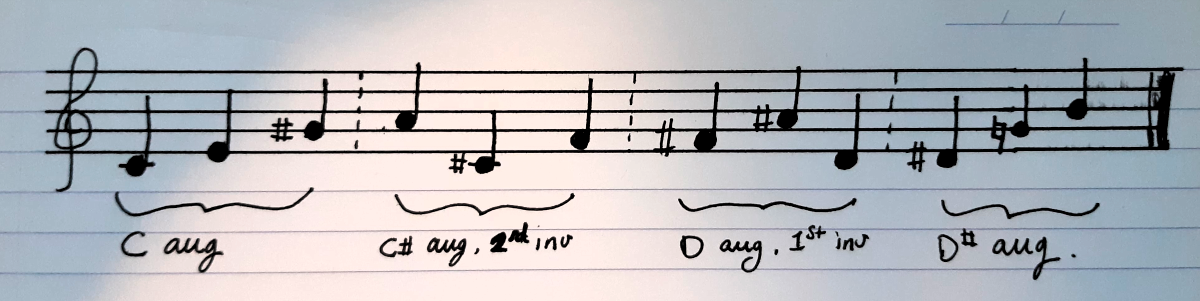
\includegraphics[width=40em]{Pictures/AppegioLikeScale.png}
 \caption{Appegio-like scale representing an order on $\bb{Z}_{12}$}
\end{figure}
In this way, the elements of $\bb{Z}_{12}$ are interpreted as the 12 tones of an octave (under standard tuning), and $n < m$ means $n$ comes before $m$ in the scale. See \cite[\S6.8.1]{Mazzola} for more details.\\\\
%
The motivating question of this project is the following:
\begin{question}
 Are there any links between fundamental \emph{computational} concepts and music?
\end{question}
 The first investigation will be on computation and \emph{musical composition}. The formal objects on the side of musical composition will be \emph{global compositions}, due to Mazzola \cite{Mazzola}. In short, a global composition consists of a collection of \emph{local compositions}, ie, small musical snippets, along with \emph{glueing instructions} describing how these snippets fit together. The guiding intuition which will relate this to computation is that just as a musical composer begins with a collection of motifs and organises them into a cohesive whole, a program consists of a collection of smaller programs which are slotted together. In other words, once a musical structure of a particular piece (ie, a global composition) has been written, appropriate local compositions can be \emph{substituted} in to \emph{realise} a complete piece. Since the language of substitution naturally arise here, we adopt the $\lambda$-calculus as our formalisation of a \emph{program}. Indeed, the ultimate goal is an appropriate category of \emph{global compositions} lying on the musical side, and an equivalence of categories between this and $\scr{L}_Q$ \cite{MurfetTroiani}, an appropriate category of $\lambda$-terms.
